\documentclass{standalone}
\usepackage{pgfplots}
\pgfplotsset{compat=1.18}
\usepgfplotslibrary{groupplots,fillbetween}
\begin{document}
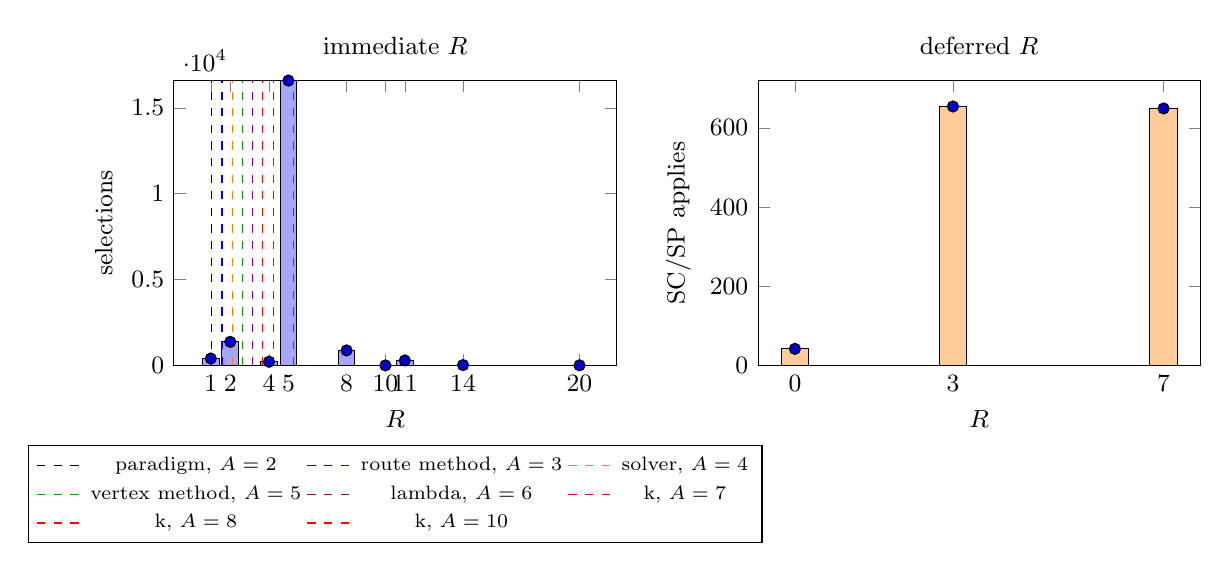
\begin{tikzpicture}
\begin{groupplot}[
  group style={group size=2 by 1, horizontal sep=1.8cm},
  width=7.2cm, height=5.2cm,
  ymin=0,
  tick label style={font=\small},
  label style={font=\small},
  title style={font=\small},
]
\nextgroupplot[title={immediate $R$}, xlabel={$R$}, ylabel={selections}, xtick={1,2,4,5,8,10,11,14,20}, ymax=16591, legend style={font=\scriptsize, at={(0.5,-0.28)}, anchor=north, legend columns=3},
  clip=false]
\addplot+[ybar, fill=blue!35, draw=black, bar width=6pt, forget plot] coordinates {(1, 407) (2, 1376) (4, 218) (5, 16591) (8, 879) (10, 5) (11, 292) (14, 25) (20, 10)};
\addplot[dashed, thin, black] coordinates {(1.0526, 0) (1.0526, 16591)};
\addlegendentry{paradigm, $A=2$}
\addplot[dashed, thin, blue] coordinates {(1.5789, 0) (1.5789, 16591)};
\addlegendentry{route method, $A=3$}
\addplot[dashed, thin, orange] coordinates {(2.1053, 0) (2.1053, 16591)};
\addlegendentry{solver, $A=4$}
\addplot[dashed, thin, green!60!black] coordinates {(2.6316, 0) (2.6316, 16591)};
\addlegendentry{vertex method, $A=5$}
\addplot[dashed, thin, violet] coordinates {(3.1579, 0) (3.1579, 16591)};
\addlegendentry{lambda, $A=6$}
\addplot[dashed, thin, red] coordinates {(3.6842, 0) (3.6842, 16591)};
\addlegendentry{k, $A=7$}
\addplot[dashed, thin, red] coordinates {(4.2105, 0) (4.2105, 16591)};
\addlegendentry{k, $A=8$}
\addplot[dashed, thin, red] coordinates {(5.2632, 0) (5.2632, 16591)};
\addlegendentry{k, $A=10$}
\nextgroupplot[title={deferred $R$}, xlabel={$R$}, ylabel={SC/SP applies}, xtick={0,3,7}]
\addplot+[ybar, fill=orange!40, draw=black, bar width=10pt] coordinates {(0, 42) (3, 654) (7, 649)};
\end{groupplot}
\end{tikzpicture}
\end{document}
